\newpage
	\section{Листок 3}
		\subsection*{Задача 1}
			\subsubsection*{\textbf{А}}
			\textbf{Условие}\\
			Докажите, что $M$ гомеоморфно ленте Мебиуса и гомотопически эквивалентно окружности.\\
			\\
			\textbf{Решение}\\
			Сперва докажем гомотопическую эквивалентность ленты Мебиуса и $S^{1}$, а потом гомеоморфизм $M$ и ленты Мебиуса.\\
			\\
			Ленту Мебиуса можно представить как квадрат $[0,1] \times [0,1]$, определенный на концах $0 \times [0,1]$ и $1 \times [0,1]$ как $(0, x) \sim (1,1 - x)$. Теперь мы можем сжимать эту группу, чтобы получить круг. Таким образом, имеется деформационный ретракт $f_t:\: M_0 \to M_0,\ t\in I$, где $M_0$ -- лента Мебиуса, такой что $f_0$ -- тождественное отображение на $M_0,\ f_1(M_0) = S^1$ и $f_t(s) = s$ для всех $s \in S^1$ и $t \in I$.\\			
			Пусть теперь $g:\ S^1 \to M_0$ -- отображение вложения. Пусть $h:\ M_0 \to S^1$ -- такое отображение, что $h = f_1$. Тогда $h \circ g = \text{id}_{S^1}$ и $f_0\simeq f_1,\ f_1 \simeq f_0$. Заметим, что $f_1:\ M_0 \to M_0$ эквивалентно $g \circ h:\ M_0 \to M_0$. Тогда, у нас есть $g \circ h \simeq f_0$ -- тождественное отображение на $M_0$. Откуда $M_0 \simeq S_1$ по определению.\\
			\\
			Теперь построим гомеоморфизм между $M$ и лентой Мебиуса\\
			Заметим, что $M$ это $\text{RP}2$ с дыркой, так как $\text{RP}2$ мы можем определить как множество всех прямых, проходящих через $(0,0,0)$, тогда строится биекция прямых с поверхностью сферы(так как прямая задается по точке пересечения со сферой), а дыркой является шапка, срезанная ограничением $z \leqslant \frac{1}{2}$, тогда необходимо доказать гомеоморфность $\text{RP}2$ с дыркой и ленты мебиуса.\\
			\\
			1) А.Л.Городенцев -- ``Линейная алгебра и геометрия'' , 2020, 17 лекция, стр. 203\\
			\\
			2) Докажем более общий случай $\mathbb{R} P^{n}=\mathbb{R}^{n} \cup \mathbb{R} P^{n-1}$ определим функцию $i: \mathbb{R}^{n} \rightarrow \mathbb{R} P^{n}$ определенную как $i\left(x_{1}, x_{2}, \dots, x_{n}\right)=\left[1, x_{1}, x_{2}, \dots, x_{n}\right]$. Тогда образ $i\left(\mathbb{R}^{n}\right)$ в $\mathbb{R} P^{n}$
			\begin{gather*}
				\left\{\left[0, x_{1}, x_{2}, \ldots, x_{n}\right] |\left(x_{1}, x_{2}, \ldots, x_{n}\right) \in \mathbb{R}^{n} \backslash\{0\}\right\} \cong \mathbb{R} P^{n-1}
			\end{gather*}
			Тогда в нашем случае $\mathbb{R} P^{2}=\mathbb{R}^{2} \cup \mathbb{R} P^{1}$, где $\mathbb{R} P^{1}$ уже определен как $S^{1}$. Теперь рассмотрим круги, заданные $[1, r \cos \phi, r \sin \phi]$. Предположим $r \rightarrow \infty$, круг удвоит покрытие $\mathbb{R} P^{1} \cong S^{1}$. Это дает необходимое разложение
			\begin{gather*}
				\mathbb{R} P^{2}=\{[1, r \cos \phi, r \sin \phi] | 0 \leq r \leq 1 \text { и } \phi \in[0,2 \pi)\}\\				
				\cup\{[r, \cos \phi, \sin \phi] | 0 \leq r \leq 1 \text { и } \phi \in[0,2 \pi)\}	
			\end{gather*}
			Где два компонента отождествляются с закрытым диском $D^{2}$ и лентой Мебиуса $M$, с общей границей $S^{1}$.\\
			
			\subsubsection*{\textbf{Б}}
			\textbf{Условие}\\
			Пусть $\iota: M \rightarrow \mathbb{R} P^{2}$ тавтологическое вложение ( $l(a)=a \in \mathbb{R} P^2$ для всякой точки $a \in M \subset \mathbb{R} P^{2}$). Вычислите гомоморфизм групп $\iota_{*}: \pi_{1}(M) \rightarrow \pi_{1}\left(\mathbb{R} P^{2}\right)$ (т.е. сначала найдите группу $\pi_1(M)$; группа $\pi_1(\mathbb{R}P^2)$ вычислялась на лекциях. После этого для каждого элемента $x \in \pi_{1}(M)$ укажите явно элемент $\iota_{*}(x) \in \pi_{1}\left(\mathbb{R} P^{2}\right)$.\\
			\\
			\textbf{Решение}\\
			\\
			Найдем фундаментальную группу $M$. $M$ гомеоморфно ленте Мебиуса $M_0$.\\			
			рассмотрим $M_0$. так как средняя линия ленты мебиуса -- строгий деформационный ретракт (мы это доказывали в 1а, но можно привести еще одно доказательство$^{\star}$), а деформационная ретрация является гомотопической эквивалентностью (так как по определению $\text{p:}\: X \to A,\ \text{in:}\: A \to X,\ \text{in} \cdot \text{p} \sim \text{id}_x$ (гомотопно)), то $	\pi_1(M_0) \sim \pi_1(S^1) \sim \mathbb{Z}$. Получаем отображение $f:\ Z \to Z/2Z,\ f(2x)=0,\ f(2x+1)=1$\\
			\\ 
			$(\star)$\\
			Докажем, что средняя линия $L$ ленты Мёбиуса $M_0$ является её строгим деформационным ретрактом. Геометричесое рассуждение очевидно: в качестве $h_t$ можно взять сжатие с коэффициентом $1-t$ ленты Мёбиуса по направлению к ее средней линии. Таким образом $h_0$ тождественно, а $h_1$ отображает $M_0$ в $L$. Выпишем формулы, так как $M_0$ -- факторпространство квадрата, то рассмотрим гомотопию
			\begin{gather*}
				H:\ I \times I \times I \to I \times I:\ (u,v,t) \to (u, (1-t)v + \frac{t}{2})
			\end{gather*}
			При этом 
			\begin{gather*}
				\forall I\quad H(u, \frac{1}{2}, t) = (u, \frac{1}{2})
			\end{gather*}
			И так как
			\begin{gather*}
				(1-t)v + \frac{t}{2} + (1-t)(1-v) + \frac{t}{2} = 1
			\end{gather*}
			То эта гомотопия выдерживает факторизацию, порождая гомотопию
			\begin{gather*}
				h:\ M_0 \times I \to M_0
			\end{gather*}
			Имеем
			\begin{gather*}
				H(u,v,0) = (u,v)
			\end{gather*}
			Откуда
			\begin{gather*}
				h_0 = \text{id}_{M_0}\\
				H_1(u,v) = (u, \frac{1}{2})
			\end{gather*}
			$(\star)$\\
			Чтобы доказать что средняя линия ленты мебиуса это деформационный ретракт ленты мебиуса, определим fundamental square как $[0,1] \times[0,1]$ со сторонами $\{0\} \times[0,1]$ и $\{1\} \times[0,1]$ соединенными: $(0, t) \sim(1,1-t)$\\
			\\
			Построим деформационный ретракт этого квадрата на интервал $[0,1] \times\{\frac{1}{2}\}$ через отображение $F((x, y), t)=(x, \frac{t}{2}+(1-t) y)$. Тогда $[0,1] \times\{\frac{1}{2}\} /(0,\frac{1}{2}) \sim(1,\frac{1}{2}) \cong S^{1}$\\
			
		\subsection*{Задача 2}
			\subsubsection*{\textbf{А}}
			\textbf{Условие}\\
			Топологическое пространство $Y_{3} \stackrel{\text { def }}{=}\left\{\left(u_{1}, u_{2}, u_{3}\right), u_{1}, u_{2}, u_{3} \in \mathbb{R}^{2} | u_{1} \neq u_{2} \neq u_{3} \neq u_{1}\right\}$. На нем действует группа перестановок $S_3$: если $\sigma \in S_3$ перестановка чисел $1,2,3$ , то отображение $R_{\sigma}:\ Y_3 \to Y_3$ определено формулой $R_{\sigma}\left(u_{1}, u_{2}, u_{3}\right) \stackrel{\text { def }}{=}\left(u_{\sigma(1)}, u_{\sigma(2)}, u_{\sigma(3)}\right)$. Пусть $X_3$ -- фактор $Y_3$ по действию
			группы (две тройки $\left(a_{1}, b_{1}, c_{1}\right),\left(a_{2}, b_{2}, c_{2}\right) \in Y_{3}$ эквивалентны, если отличаются только порядком точек). Докажите, что отображение проекции $p: Y_{3} \rightarrow X_{3}$ -- накрытие.
			\\
			\textbf{Решение}\\
			Определение накрытия:\\
			$p: Y_3 \to X_3$ непрерывно, сюръективно и $\forall\ V \in X_3\ \exists v \in V$ -- окрестеность, такая что $p^{-1}(U)$ представляется в виде $U$ непересекающихся открытых множеств $V_{\alpha}$, каждое из кторых гомеоморфно отображению на $U$
			\begin{gather*}
				Y_3 = \{(u_1,u_2,u_3)\ |\ u_1,u_2,u_3 \in \mathbb{R}\ |\ u_1 \ne u_2 \ne u_3 \ne u_1\}
			\end{gather*}
			окрестность элемента $u \in Y_3:\ U = U_1 \times U_2 \times U_3,\ u_i \in U_i$\\
			Так как $\mathbb{R}^2$ -- хаусдорфово, то для $u_1 \ne u_2 \ne u_3 \ne u_1$	существуют непересекающиеся окрестности $U_1,U_2,U_3$\\
			Теперь рассмотрим $p^{-1}(v)=(v_1,v_2,v_3),\ V=(v_1,v_2,v_3)$ с точностью до перестановки, то есть $p^{-1}(V) = \bigcup\limits^{3}_{\underset{i \ne j \ne k\ne i}{i,j,k = 1}} V_i \times V_j \times V_k$ -- непересекающиеся открытые множества из $Y_3$, тогда $p$ является накрытием по определению\\
			\begin{comment}
			Заметим, что $Y_3$ -- наборы из 3 различных точек с учетом порядка, а $X_3$ -- наборы из 3 различных точек без учета порядка. Тогда проекция сопоставляет наборы с учетом поряда точек, набору без учета этого порядка (то есть наборам $a_1a_2a_3,\ a_1a_3a_2,\ a_2a_1a_3,\ a_2a_3a_1,\ a_3a_1a_2,\ a_3a_2a_1$ мы сопоставляем множество $\{a_1, a_2, a_3\}$). Тогда рассмотрим что является прообразом окрестности $B$, точки $\{a_1,a_2,a_3\}$, в $Y_3$. Определим окрестность набора точек $a_1a_2a_3$ как произведение их окретностей из $\mathbb{R}^2$, то есть $b_1b_2b_3$ лежит в окрестности $u$ набора $a_1a_2a_3$ только если $b_1$ лежит в окрестности $a_1$ в $\mathbb{R}^2$, $b_2$ лежит в окрестности $a_2$ в $\mathbb{R}^2$ и $b_3$ лежит в окрестности $a_3$ в $\mathbb{R}^2$. Представим последовательность точек $a_1a_2a_3$ как точку из $\mathbb{R}^6$, у которой первые 2 координыта совпадают с первым элементом последовательности, следующие две со вторым и последние две с третьим. Тогда если рассмотреть точку $x_1x_2x_3 \in X_3$, то прообраз её окрестности $p^{-1}(u)$ (где $u$ -- окрестность) является объединением непересекакющихся окрестностей точек $a_1a_2a_3,\ a_1a_3a_2,\ a_2a_1a_3,\ a_2a_3a_1,\ a_3a_1a_2,\ a_3a_2a_1$, расположенных в $\mathbb{R}^6$, тогда это отображение является накрытием по определению.	
			\end{comment}
			
			
			\subsubsection*{\textbf{Б}}
			\textbf{Условие}\\
			Пусть $u \in Y_{3}$ -- какая-то точка, и $v \stackrel{\text { def }}{=} p(u) \in X_{3}$. Рассмотрим петлю $\gamma:[0,1] \rightarrow X_{3}$ такую, что $\gamma(0)=\gamma(1)=v$, и пусть $\Gamma:[0,1] \rightarrow Y_{3}$ -- ее поднятие с начальной точкой $\Gamma(0)=u$. Обозначим $\sigma \in S_{3}$ перестановку, для которой $\Gamma(1)=R_{\sigma}(u)$. Докажите, что соответствие $\gamma \mapsto \sigma^{-1}$ -- гомоморфизм групп $\pi_{1}\left(X_{3}, v\right) \rightarrow S_{3}$.\\
			\\
			\textbf{Решение}\\
			\begin{gather*}
				u \in Y_3\\
				\Gamma(0) = u\\
				\Gamma(1) = \mathbb{R}_{\sigma}(u)\\
				v = p(u) \in X_3\\
				\gamma(0) = \gamma(1) = v
			\end{gather*}
			\begin{wrapfigure}{h}{0.2\textwidth}
				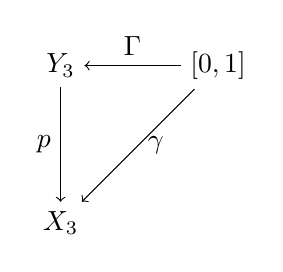
\begin{tikzpicture}[node distance=2cm, auto]
				\node (X) {$Y_3$};
				\node(Y) [right of=X] {$[0,1]$};
				\node (X1) [below of=X] {$X_3$};
				\draw[->](X) to node [left]{$p$}(X1);
				\draw[<-](X1) to node [right]{$\gamma$}(Y);
				\draw[<-](X) to node {$\Gamma$}(Y);
				\end{tikzpicture}
			\end{wrapfigure}
			Лемма о накрывающем пути:\\
			$\forall$ пути $s: I \to X_3$, начинающемся в $v$,\\
			$\exists!$ путь $\tilde{s}: I \to Y_3$, начинающийся в $u$ и накрывающий $s$\\
			То есть 
			\begin{gather*}
				\exists\ \tilde{s}: I \to X_3\quad \gamma(0) = \gamma(1) = v\quad \exists!\ \Gamma: I \to Y_3\ |\ \Gamma(0) = u\\
			\end{gather*}
			Следовательно $\pi_1(X_3,v)$ состоит из петель $\gamma_i$, которым однозначно соответствуют $\sigma_i\ \Rightarrow$ соответствуют $\sigma^{-1}_i$\\
			(так как $\forall\ \sigma_i\ \exists!\ \sigma^{-1}_i\ |\ \sigma_i \cdot \sigma^{-1}_i = \sigma^{-1}_i \cdot \sigma_i = \text{id}$)\\
			\begin{gather*}
				\pi_1(X_3,v) \overset{f}{\to} S_3\\
				\gamma \overset{f}{\to} \sigma^{-1}\\
				f(\gamma_i) = f(p(R_{\sigma_i}(u))) = \sigma^{-1}_i\\
				f(\gamma_1) \cdot f(\gamma_2) = f(p(R_{\sigma_1}(u))) \cdot f(p(R_{\sigma_2}(u))) = fp(u_{\sigma_1(1)}, u_{\sigma_1(2)}, u_{\sigma_1(3)}) \times fp(u_{\sigma_2(1)}, u_{\sigma_2(2)}, u_{\sigma_2(3)}) = (1)
			\end{gather*}
			Так как $\sigma_1 \cdot \sigma_2 = p(R_{\sigma_1}(u) \cdot R_{\sigma_2}(u))$ то
			\begin{gather*}
				(1) = fp(u_{\sigma_2\sigma_1(1)}, u_{\sigma_2\sigma_1(2)}, u_{\sigma_2\sigma_1(3)}) = fp(R_{\sigma_2\sigma_1}(u)) = (\sigma_2\sigma_1)^{-1} = \sigma_1^{-1} \sigma_2^{-1}
			\end{gather*}
			То есть это гомоморфизм, что и требовалось доказать.
			\\
			
			\subsubsection*{\textbf{В}}
			\textbf{Условие}\\
			Докажите, что группа $\pi_{1}\left(X_{3}, v\right)$ некоммутативна\\
			\\
			\textbf{Решение}\\
			рассмотрим перестановки $\sigma_1 = (1,3)(2),\ \sigma_2 = (3,1,2)$\\
			Тогда
			\begin{gather*}
				\sigma_1 \cdot \sigma_2 = (12)(3)\\
				\sigma_2 \cdot \sigma_1 = (123)\\
				\sigma_1 \cdot \sigma_2 \ne \sigma_2 \cdot \sigma_1\\
				\gamma_1 \cdot \gamma_2 \ne \gamma_2 \cdot \gamma_1
			\end{gather*}
			Откуда следует что группа $\pi_1(X_3,v)$ некоммутативна
			\\
			